\documentclass{ximera}  


%\usepackage{todonotes}
%\usepackage{mathtools} %% Required for wide table Curl and Greens
%\usepackage{cuted} %% Required for wide table Curl and Greens
\newcommand{\todo}{}

\usepackage{esint} % for \oiint
\ifxake%%https://math.meta.stackexchange.com/questions/9973/how-do-you-render-a-closed-surface-double-integral
\renewcommand{\oiint}{{\large\bigcirc}\kern-1.56em\iint}
\fi


\graphicspath{
  {./}
  {jpg}
  {ximeraTutorial/}
  {basicPhilosophy/}
  {functionsOfSeveralVariables/}
  {normalVectors/}
  {lagrangeMultipliers/}
  {vectorFields/}
  {greensTheorem/}
  {shapeOfThingsToCome/}
  {dotProducts/}
  {partialDerivativesAndTheGradientVector/}
  {../productAndQuotientRules/exercises/}
  {../motionAndPathsInSpace/exercises/}
  {../normalVectors/exercisesParametricPlots/}
  {../continuityOfFunctionsOfSeveralVariables/exercises/}
  {../partialDerivativesAndTheGradientVector/exercises/}
  {../directionalDerivativeAndChainRule/exercises/}
  {../commonCoordinates/exercisesCylindricalCoordinates/}
  {../commonCoordinates/exercisesSphericalCoordinates/}
  {../greensTheorem/exercisesCurlAndLineIntegrals/}
  {../greensTheorem/exercisesDivergenceAndLineIntegrals/}
  {../shapeOfThingsToCome/exercisesDivergenceTheorem/}
  {../greensTheorem/}
  {../shapeOfThingsToCome/}
  {../separableDifferentialEquations/exercises/}
  {vectorFields/}
}

\newcommand{\mooculus}{\textsf{\textbf{MOOC}\textnormal{\textsf{ULUS}}}}

\usepackage{tkz-euclide}\usepackage{tikz}
\usepackage{tikz-cd}
\usetikzlibrary{arrows}
\tikzset{>=stealth,commutative diagrams/.cd,
  arrow style=tikz,diagrams={>=stealth}} %% cool arrow head
\tikzset{shorten <>/.style={ shorten >=#1, shorten <=#1 } } %% allows shorter vectors

\usetikzlibrary{backgrounds} %% for boxes around graphs
\usetikzlibrary{shapes,positioning}  %% Clouds and stars
\usetikzlibrary{matrix} %% for matrix
\usepgfplotslibrary{polar} %% for polar plots
\usepgfplotslibrary{fillbetween} %% to shade area between curves in TikZ
\usetkzobj{all}
\usepackage[makeroom]{cancel} %% for strike outs
%\usepackage{mathtools} %% for pretty underbrace % Breaks Ximera
%\usepackage{multicol}
\usepackage{pgffor} %% required for integral for loops



%% http://tex.stackexchange.com/questions/66490/drawing-a-tikz-arc-specifying-the-center
%% Draws beach ball
\tikzset{pics/carc/.style args={#1:#2:#3}{code={\draw[pic actions] (#1:#3) arc(#1:#2:#3);}}}



\usepackage{array}
\setlength{\extrarowheight}{+.1cm}
\newdimen\digitwidth
\settowidth\digitwidth{9}
\def\divrule#1#2{
\noalign{\moveright#1\digitwidth
\vbox{\hrule width#2\digitwidth}}}





\newcommand{\RR}{\mathbb R}
\newcommand{\R}{\mathbb R}
\newcommand{\N}{\mathbb N}
\newcommand{\Z}{\mathbb Z}

\newcommand{\sagemath}{\textsf{SageMath}}


%\renewcommand{\d}{\,d\!}
\renewcommand{\d}{\mathop{}\!d}
\newcommand{\dd}[2][]{\frac{\d #1}{\d #2}}
\newcommand{\pp}[2][]{\frac{\partial #1}{\partial #2}}
\renewcommand{\l}{\ell}
\newcommand{\ddx}{\frac{d}{\d x}}

\newcommand{\zeroOverZero}{\ensuremath{\boldsymbol{\tfrac{0}{0}}}}
\newcommand{\inftyOverInfty}{\ensuremath{\boldsymbol{\tfrac{\infty}{\infty}}}}
\newcommand{\zeroOverInfty}{\ensuremath{\boldsymbol{\tfrac{0}{\infty}}}}
\newcommand{\zeroTimesInfty}{\ensuremath{\small\boldsymbol{0\cdot \infty}}}
\newcommand{\inftyMinusInfty}{\ensuremath{\small\boldsymbol{\infty - \infty}}}
\newcommand{\oneToInfty}{\ensuremath{\boldsymbol{1^\infty}}}
\newcommand{\zeroToZero}{\ensuremath{\boldsymbol{0^0}}}
\newcommand{\inftyToZero}{\ensuremath{\boldsymbol{\infty^0}}}



\newcommand{\numOverZero}{\ensuremath{\boldsymbol{\tfrac{\#}{0}}}}
\newcommand{\dfn}{\textbf}
%\newcommand{\unit}{\,\mathrm}
\newcommand{\unit}{\mathop{}\!\mathrm}
\newcommand{\eval}[1]{\bigg[ #1 \bigg]}
\newcommand{\seq}[1]{\left( #1 \right)}
\renewcommand{\epsilon}{\varepsilon}
\renewcommand{\phi}{\varphi}


\renewcommand{\iff}{\Leftrightarrow}

\DeclareMathOperator{\arccot}{arccot}
\DeclareMathOperator{\arcsec}{arcsec}
\DeclareMathOperator{\arccsc}{arccsc}
\DeclareMathOperator{\si}{Si}
\DeclareMathOperator{\scal}{scal}
\DeclareMathOperator{\sign}{sign}


%% \newcommand{\tightoverset}[2]{% for arrow vec
%%   \mathop{#2}\limits^{\vbox to -.5ex{\kern-0.75ex\hbox{$#1$}\vss}}}
\newcommand{\arrowvec}[1]{{\overset{\rightharpoonup}{#1}}}
%\renewcommand{\vec}[1]{\arrowvec{\mathbf{#1}}}
\renewcommand{\vec}[1]{{\overset{\boldsymbol{\rightharpoonup}}{\mathbf{#1}}}\hspace{0in}}

\newcommand{\point}[1]{\left(#1\right)} %this allows \vector{ to be changed to \vector{ with a quick find and replace
\newcommand{\pt}[1]{\mathbf{#1}} %this allows \vec{ to be changed to \vec{ with a quick find and replace
\newcommand{\Lim}[2]{\lim_{\point{#1} \to \point{#2}}} %Bart, I changed this to point since I want to use it.  It runs through both of the exercise and exerciseE files in limits section, which is why it was in each document to start with.

\DeclareMathOperator{\proj}{\mathbf{proj}}
\newcommand{\veci}{{\boldsymbol{\hat{\imath}}}}
\newcommand{\vecj}{{\boldsymbol{\hat{\jmath}}}}
\newcommand{\veck}{{\boldsymbol{\hat{k}}}}
\newcommand{\vecl}{\vec{\boldsymbol{\l}}}
\newcommand{\uvec}[1]{\mathbf{\hat{#1}}}
\newcommand{\utan}{\mathbf{\hat{t}}}
\newcommand{\unormal}{\mathbf{\hat{n}}}
\newcommand{\ubinormal}{\mathbf{\hat{b}}}

\newcommand{\dotp}{\bullet}
\newcommand{\cross}{\boldsymbol\times}
\newcommand{\grad}{\boldsymbol\nabla}
\newcommand{\divergence}{\grad\dotp}
\newcommand{\curl}{\grad\cross}
%\DeclareMathOperator{\divergence}{divergence}
%\DeclareMathOperator{\curl}[1]{\grad\cross #1}
\newcommand{\lto}{\mathop{\longrightarrow\,}\limits}

\renewcommand{\bar}{\overline}

\colorlet{textColor}{black}
\colorlet{background}{white}
\colorlet{penColor}{blue!50!black} % Color of a curve in a plot
\colorlet{penColor2}{red!50!black}% Color of a curve in a plot
\colorlet{penColor3}{red!50!blue} % Color of a curve in a plot
\colorlet{penColor4}{green!50!black} % Color of a curve in a plot
\colorlet{penColor5}{orange!80!black} % Color of a curve in a plot
\colorlet{penColor6}{yellow!70!black} % Color of a curve in a plot
\colorlet{fill1}{penColor!20} % Color of fill in a plot
\colorlet{fill2}{penColor2!20} % Color of fill in a plot
\colorlet{fillp}{fill1} % Color of positive area
\colorlet{filln}{penColor2!20} % Color of negative area
\colorlet{fill3}{penColor3!20} % Fill
\colorlet{fill4}{penColor4!20} % Fill
\colorlet{fill5}{penColor5!20} % Fill
\colorlet{gridColor}{gray!50} % Color of grid in a plot

\newcommand{\surfaceColor}{violet}
\newcommand{\surfaceColorTwo}{redyellow}
\newcommand{\sliceColor}{greenyellow}




\pgfmathdeclarefunction{gauss}{2}{% gives gaussian
  \pgfmathparse{1/(#2*sqrt(2*pi))*exp(-((x-#1)^2)/(2*#2^2))}%
}


%%%%%%%%%%%%%
%% Vectors
%%%%%%%%%%%%%

%% Simple horiz vectors
\renewcommand{\vector}[1]{\left\langle #1\right\rangle}


%% %% Complex Horiz Vectors with angle brackets
%% \makeatletter
%% \renewcommand{\vector}[2][ , ]{\left\langle%
%%   \def\nextitem{\def\nextitem{#1}}%
%%   \@for \el:=#2\do{\nextitem\el}\right\rangle%
%% }
%% \makeatother

%% %% Vertical Vectors
%% \def\vector#1{\begin{bmatrix}\vecListA#1,,\end{bmatrix}}
%% \def\vecListA#1,{\if,#1,\else #1\cr \expandafter \vecListA \fi}

%%%%%%%%%%%%%
%% End of vectors
%%%%%%%%%%%%%

%\newcommand{\fullwidth}{}
%\newcommand{\normalwidth}{}



%% makes a snazzy t-chart for evaluating functions
%\newenvironment{tchart}{\rowcolors{2}{}{background!90!textColor}\array}{\endarray}

%%This is to help with formatting on future title pages.
\newenvironment{sectionOutcomes}{}{}



%% Flowchart stuff
%\tikzstyle{startstop} = [rectangle, rounded corners, minimum width=3cm, minimum height=1cm,text centered, draw=black]
%\tikzstyle{question} = [rectangle, minimum width=3cm, minimum height=1cm, text centered, draw=black]
%\tikzstyle{decision} = [trapezium, trapezium left angle=70, trapezium right angle=110, minimum width=3cm, minimum height=1cm, text centered, draw=black]
%\tikzstyle{question} = [rectangle, rounded corners, minimum width=3cm, minimum height=1cm,text centered, draw=black]
%\tikzstyle{process} = [rectangle, minimum width=3cm, minimum height=1cm, text centered, draw=black]
%\tikzstyle{decision} = [trapezium, trapezium left angle=70, trapezium right angle=110, minimum width=3cm, minimum height=1cm, text centered, draw=black]




 
\title{Biot-Savart's Law} 
\author{Milica Markovic} 
\outcome{Use Bio-Savart's Law to calculate magnetic field due to a current distribution.}
\begin{document}  
\begin{abstract}  

\end{abstract}  
\maketitle    


\section{Magnetic Field due to a Charge Distribution}






We will first find the magnetic field due to a loop carrying current $I$,  positioned in the X-Y plane, as shown in Figure \ref{fig:magfield}. To solve this problem, we will first divide the loop into small pieces and label one of these pieces as $dl$. The magnetic field due to an infinitesimal current, can be found using Biot-Savart's law. Magnetic field is labeled in Figure \ref{fig:magfield} as $dB$.  The infinitesimal current position is defined by a position vector $\vec{r_2}$. The position of point P, where the field will be calculated,  is defined with the position vector  $\vec{r_1}$. The distance between the current and the observation point is labeled as $\vec{r}$. The vector  $\vec{dB}$ is defined in  Equation  \ref{bscur}.


\begin{eqnarray}
\vec{dB_l}=\frac{\mu \,I }{4 \pi r^3} (\hat{dl} \times \hat{r})\label{bscur}
\end{eqnarray}


\begin{figure}[htbp]
\begin{center}
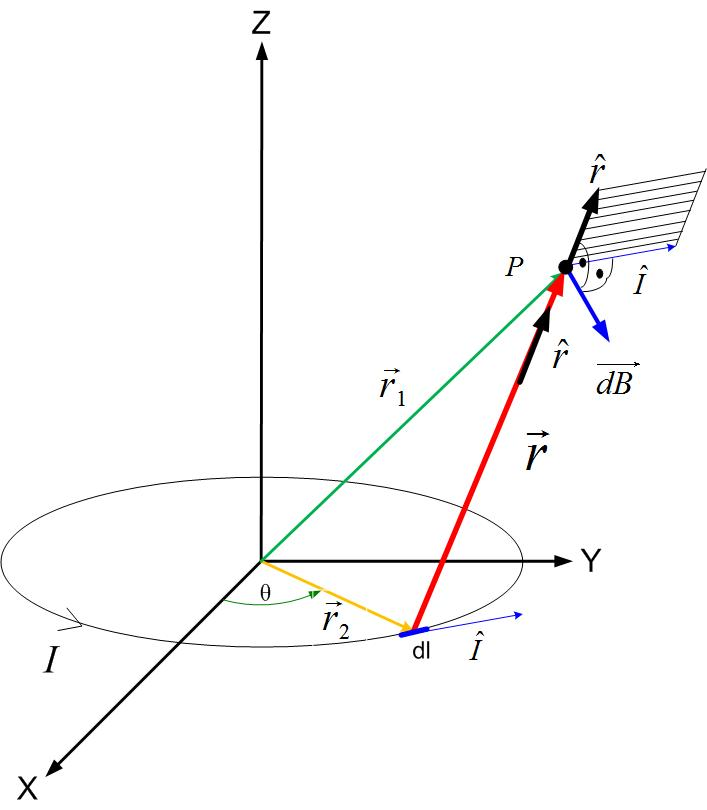
\includegraphics[scale=0.3]{../jpg/magfieldloop.jpg}
%\strut\psfig{figure=chargedistribution.ps,width=3cm} \\
\end{center}
\caption{Loop of wire carrying current $I$. Magnetic  field is shown due to a very small section (arc length) of the loop $dl$.}
\label{fig:magfield}
\end{figure}

The total magnetic field at a point P is then equal to the sum of all the fields due to the elemental currents, as shown in Figure \ref{bscur1}. The equation for the total field is given in \ref{eqtotfieldringm}. 

\begin{eqnarray}
\vec{B}=\int\limits_{all \,\, inf. \,\, currents} \vec{dB} \label{eqtotfieldringm}
\end{eqnarray}

\begin{figure}[htbp]
\begin{center}
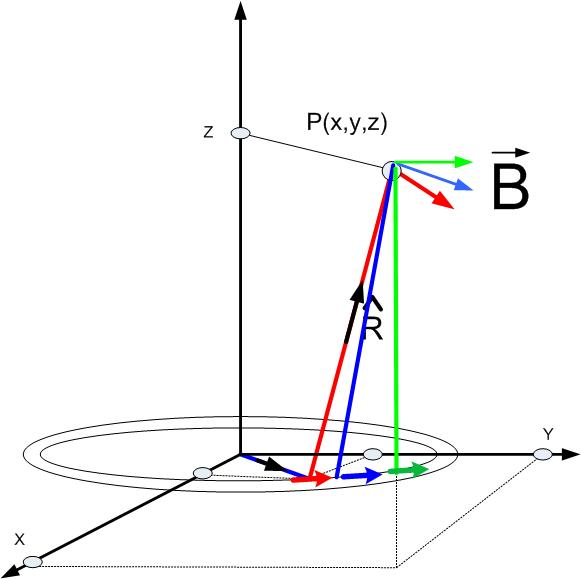
\includegraphics[scale=0.4]{../jpg/bscurrent.jpg}
%\strut\psfig{figure=bscurrent.ps,width=3cm} \\
\end{center}
\caption{Loop of wire uniformly charged with line charge density $\rho_l$. Electric field is shown due to several very small sections (arc length) of the loop $dl$.
Each section is modeled by a point charge $dQ$.}
\label{bscur1}
\end{figure}



The problem now  is to represent all the variables in the Equation \ref{bscur}  ( $I$, $dl$, $\hat{r}$ and $r$) using  appropriate coordinate system and given current distribution.
 As seen in Figure \ref{fig:magfield}, $\vec{dl}$ is an arc length in the direction of theta (blue arrow next to $dl$) $dl=a\, d\theta a_{\theta}$, where $ a$ is the radius of the loop. The vector $\vec{r_2}$ is the position vector of the arc length $dl$, and the vector $\vec{r_1}$  is the position vector of the point P where we want the find the magnetic field. Point P is an arbitrary point in the Cartesian coordinate system, P(x,y,z), therefore its vector is shown in Equation\ref{eq1loopm}.  The vector $\vec{r}$ is the distance vector between the elemental current (the source) and the point at which we are calculating the electric field. 



\begin{eqnarray}
\vec{r_1}=x \vec{a_x} + y \vec{a_y} +z\vec{a_z} \label{eq1loopm}
\end{eqnarray}

The vector $\vec{r_2}$ can be written in Polar Coordinates as in Equation \ref{pcvecm},where $a$ is the radius of the loop. The equation \ref{pcvecm} can be rewritten in Cartesian coordinate system as in Equation \ref{csloopvecm}.

\begin{eqnarray}
\vec{r_2}=a \, \vec{a_r} \label{pcvecm} \\
\vec{a_r}= \,cos{\theta} \, \vec{a_x}+ sin{\theta} \, \vec{a_y} \\
\vec{r_2}=a \, cos{\theta}\,  \vec{a_x}+ a \, sin{\theta} \, \vec{a_y} \label{csloopvecm}
\end{eqnarray}

The two vectors mark the beginning and the end of the distance vector $\vec{r}$. The vector  $\vec{r}$ is the sum of vectors $-\vec{r_2}$ and $\vec{r_1}$. 



\begin{eqnarray}
\vec{r}=\vec{r_1} + (-\vec{r_2})
\end{eqnarray}


Therefore the vector's $\vec{r}$  magnitude and the unit vector are shown in Equations \ref{vecrloop1m}-\ref{vecrloop2m}.


\begin{eqnarray}
\vec{r}= (x -  a \,cos{\theta}) \vec{a_x} +(y - a \,sin{\theta}) \vec{a_y} +z \vec{a_z}
\end{eqnarray}

Vector $\vec{r}$ has the magnitude of:


\begin{eqnarray}
|\vec{r}|= \sqrt{(x - a \,cos{\theta})^2 +(y - a \,sin{\theta})^2 +z ^2}\label{vecrloop1m}
\end{eqnarray}

Unit vector in the direction of vector $\vec{r}$ is:


\begin{eqnarray}
\hat{r}= \frac{\vec{r}}{|\vec{r}|} \\
\hat{r}=\frac{\vec{r}}{\sqrt{(x - a \, cos{\theta})^2 +(y - a  \, sin{\theta})^2 +z^2}}\label{vecrloop2m}
\end{eqnarray}

Cross product between the distance vector $\vec{r}$ and the vector of the direction of current $\hat{I}$ is found in Equations \ref{eq:cprloop}-\ref{eq:product}.

\begin{eqnarray}
\vec{dl}=  a\,  d\theta \, \vec{ a_{\theta}} \\
a_{\theta}= -\, sin\theta \, a_{x} \, + \, cos\theta \vec{a_y}  \\
\vec{dl}= -\, a \,  sin\theta \, d \theta \, \vec{a_{x}} \, + a \, cos \theta\,  d \theta \,\vec{a_y} 
\end{eqnarray}

\begin{eqnarray}\label{eq:cprloop} 
\vec{dl} \times \vec{r} = \cdots \nonumber \\ 
 \left( -\, a \,  sin\theta \, d \theta \, \vec{a_{x}} \, + a \, cos \theta\,  d \theta \,\vec{a_y}\right)  \times \left(  (x -  a \,cos{\theta}) \vec{a_x} +(y - a \,sin{\theta}) \vec{a_y} +z \vec{a_z} \right) 
\end{eqnarray}
\begin{eqnarray}\label{eq:product}
\vec{dl} \times \vec{r} =\left| \begin{array}{ccc}
\vec{a_x} & \vec{a_y} & \vec{a_z} \\
   -\, a \,  sin\theta \, d \theta &  a \, cos \theta\,  d \theta & 0 \\
 (x -  a \,cos{\theta}) & (y - a \,sin{\theta})  & z \end{array} \right| 
\end{eqnarray}

\begin{eqnarray}
dl\times \vec{r} =\cdots \nonumber \\ (z a \, cos\theta \,d\theta) \,\vec{a_x}  + (a\, z \,sin\theta \,d\theta) \,\vec{a_y} + (a^2 \,-\,a \,(y\, sin\theta\, +\, x \,cos\theta))\, d\theta \,\vec{a_z} 
\end{eqnarray}


Replacing other variables in the Equations \ref{eq1loopm}-\ref{vecrloop2m}, we get the    Equation \ref{eq:totalfieldloop1m} for the magnetic field $\vec{dB}$ at a point P.

Components of the magnetic field are given in Equations \ref{eq:totalfieldloop1m}-\ref{eq:totalfieldloop3m}.

\begin{eqnarray}
\label{eq:totalfieldloop1m} \vec{dB}_x = \frac{\mu I}{4 \pi \sqrt{(x - a \,cos{\theta})^2 +(y - a \,sin{\theta})^2 +z ^2}^3 } (z \, a \, cos\theta \, d\theta) \vec{a_x}    \\
\label{eq:totalfieldloop2m}  \vec{dB}_y= \frac{\mu I}{4 \pi \sqrt{(x - a \,cos{\theta})^2 +(y - a \,sin{\theta})^2 +z ^2}^3 } (a \, z \, sin\theta \, d\theta) \vec{a_y} \\
 \label{eq:totalfieldloop3m}\vec{dB}_z=  
\frac{\mu I}{4 \pi \sqrt{(x - a \,cos{\theta})^2 +(y - a \,sin{\theta})^2 +z ^2}^3 } \cdots \nonumber \\ \cdots (a^2 \, -\, a \, (y\,  sin\theta\, + \,x\, cos\theta)) \, d\theta \, \vec{a_z} 
\end{eqnarray}


Each field component can be integrated separately, as shown in Equations \ref{totalfieldloop4m}-\ref{totalfieldloop6m}.



\begin{eqnarray}
\vec{B_x}= \int_0^{2\pi}\frac{\mu\,  I\,  z\,  a\,  cos\theta \, d\theta}{4 \, \pi\,  \sqrt{(x\,  - \, a \,cos{\theta})^2 +(y \,- \,a \,sin{\theta})^2 \,+\,z ^2}^3 }  \, \vec{a_x} \label{totalfieldloop4m} \\
\vec{B_y}=  \int_0^{2\pi} \frac{\mu \, I \, a \, z\, sin\theta\, d\theta}{4\, \pi \, \sqrt{(x \,-\,  a \,cos{\theta})^2 +(y \, - \, a \,sin{\theta})^2 \,+\, z ^2}^3 }  \, \vec{a_y} \label{totalfieldloop5m} \\
\vec{B_z}=  \int_0^{2\pi} \frac{\mu  \,I(a^2 \,-\,a\, (y\, sin\theta \,+\, x\, cos\theta))\,d\theta}{4 \,\pi\, \sqrt{(x\, -\, a \,cos{\theta})^2 +(y\, -\, a \,sin{\theta})^2 \,+\,z ^2}^3 }  \vec{a_z} \label{totalfieldloop6m}
\end{eqnarray}

The magnetic field above is shown in Figure \ref{mflmat}

\begin{figure}[htbp]
\begin{center}
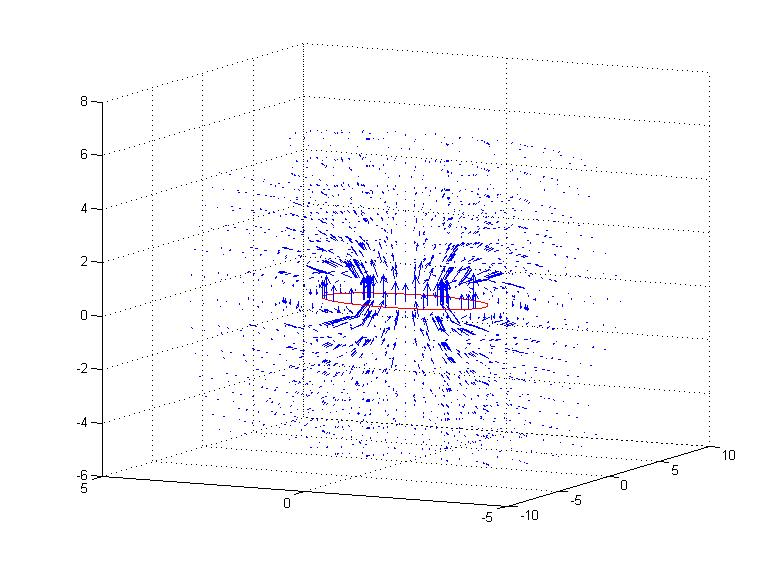
\includegraphics[scale=0.3]{../jpg/bfieldloop.jpg}
%\strut\psfig{figure=increaseinflux.ps,width=3cm} \\
\end{center}
\caption{Magnetic Field of a Loop of Current }
\label{mflmat}
\end{figure}



\section{Visualizing Scalar Fields in Matlab}

To visualize scalar fields in Matlab, we can use the following functions: slice, contourslice, patch, isonormals, camlight, and lightning. Please note that a more detailed explanation about these functions can be found in Matlab help.

\subsection{slice}
 
Slice is a command that shows the magnitude of a scalar field on a plane that slices the volume where the potential field is visualized. The format of this command is as shown below.

\begin{verbatim}
slice(x,y,z,v,xslice,yslice,zslice)
\end{verbatim}

Where X, Y, and Z are coordinates of points where the scalar function is calculated, V is v the scalar function at those points, and the last three vectors xslice, yslice, and zslice are showing where will the volume will be sliced.

An example of a slice command is given below. There is an additional command colormap that colors the volume with a specific palette in the example below. To see more about different color maps, see Matlab help. xslice has three points at which the x-axis will be slice. They are -1.2, .8, 2. The volume will be sliced with a plane perpendicular to the x-axis, and it crosses the x-axis at points -1.2, .8, and 2. 
 
\begin{verbatim}
clc
clear all
[x,y,z] = meshgrid(-2:.2:2,-2:.25:2,-2:.16:2);
v = x.*exp(-x.^2-y.^2-z.^2);
xslice = [-1.2,.8,2]; yslice = 1; zslice = [-2,0];
slice(x,y,z,v,xslice,yslice,zslice)
colormap hsv
\end{verbatim}

\subsection{contourslice}

 Contourslice command will display equipotential lines on a plane being the volume where the potential field is visualized. An example of contourslice function is shown below.

\begin{verbatim}
[x,y,z] = meshgrid(-2:.2:2,-2:.25:2,-2:.16:2);
v = x.*exp(-x.^2-y.^2-z.^2); % Create volume data
[xi,yi,zi] = sphere; % Plane to contour
contourslice(x,y,z,v,xi,yi,zi)
view(3)
\end{verbatim}

\subsection{patch}

Patch command creates a patch of color.


\subsection{isonormals}

Command isonormals creates equipotential surfaces. 
\subsection{camlight}

\begin{verbatim}
camlight('headlight') creates a light at the camera
 position.camlight('right') creates a light
right and up from camera.

camlight('left') creates a light
left and up from camera.camlight with no arguments is the
same as camlight('right').

camlight(az,el) creates a light
at the specified azimuth (az) and elevation (el)
with respect to the camera position. The camera target 
is the center of rotation
and az and el are in degrees.

\end{verbatim}



\subsection{lighting}


\begin{verbatim}
lighting flat selects flat lighting.

Lighting gouraud selects gouraud lighting.

Lighting phong selects phong lighting.

Lighting none turns off lighting.
\end{verbatim}






\end{document} 

